\chapter {Dobór danych} 
{
    Jednym z\,\,kluczowych aspektów każdego procesu analizy danych i\,\,uczenia maszynowego
    jest odpowiedni dobór danych. Decyzje podjęte na tym etapie pociągają za sobą 
    konsekwencje w\,\,kolejnych etapach procesu. W\,\,zależności od postaci danych wejściowych,
    określany jest konieczny nakład pracy w\,\,procesie ich obróbki. 
    Ponadto, odpowiedni dobór danych ma znaczący wpływ na otrzymywane wyniki.

    W\,\,przypadku danych muzycznych należy zwrócić uwagę między innymi na cechy takie jak:
    \begin{itemize}
        \setlength\itemsep{-0.5em}
        \item dostępność danych treningowych,
        \item sposób reprezentacji upływu czasu,
        \item sposób wyrażenia wysokości dźwięku,
        \item jasność przedstawiania zależności między dźwiękami,
        \item stopień kompresji,
        \item złożoność samego formatu oraz możliwość istnienia niepoprawnych reprezentacji.
    \end{itemize}

    \section{Porównanie formatów danych}
    {
        Wybór odpowiedniego formatu danych został poprzedzony analizą zbioru popularnych formatów muzycznych.
        Zbiór porównanych rodzajów plików ograniczono do plików audio, notacji ABC oraz midi.
        Opisane formaty zostały dobrane na podstawie ich odmienności względem siebie.

        \subsection{Pliki audio}
        {
            Najmniej restrykcyjnymi formatami plików audio są formaty będące zapisem
            amplitudy fali akustycznej. Przykładami plików tego rodzaju są pliki WAV
            oraz AIFF.
            Kluczowym parametrem plików audio jest częstotliwość próbkowania. Od niej
            zależy zakres możliwych do wyrażenia częstotliwości. Typową wartością dla plików
            WAV jest 44100Hz, co według twierdzenia Nyquista-Shannona przekłada się na zakres
            częstotliwości ograniczony wartością 22050Hz \cite{Shannon1949CommunicationIT}, będącą bliską granicy słyszalności
            ludzkiego aparatu słuchowego. 

            W\,\,przeciwieństwie do pozostałych opisanych formatów, wysokości dźwięków wyrażone są 
            jedynie poprzez sekwencje zmian amplitudy sygnału, przez co
            ich ekstrakcja wymagałaby wykorzystania transformaty Fouriera.

            Największą zaletą i\,\,jednocześnie wadą tego formatu jest jego swoboda. 
            Postać fali akustycznej pozwala na przedstawienie każdego dźwięku będącego w\,\,paśmie
            przenoszenia, zarówno złożonych wieloinstrumentowych kompozycji muzycznych, 
            prostych melodii, jak i\,\,dźwięków nie podlegających pod definicję muzyki. 
            Prowadzi to do niskiego stopnia kompresji informacji, wymuszającego złożone metody obróbki i\,\,skomplikowane
            modele uczenia.
        }

        \subsection{Notacja ABC}\label{chap:abc}
        {
            Notacja ABC jest jedną z\,\,cyfrowych postaci klasycznego zapisu nutowego.
            Dane w\,\,plikach ABC przedstawione są za pomocą znaków ASCII.

            Ponieważ jest to odpowiednik zapisu nutowego, oznacza to
            że zarówno wysokości dźwięków, jak i\,\,wartości rytmiczne należą do dyskretnego zbioru.
            Fakt ten nakłada spore ograniczenie na treść plików, lecz w\,\,kontekście muzyki są to 
            ograniczenia bardzo pomocne.

            Poza informacją o\,\,samym dźwięku i\,\,jego wartości rytmicznej, format zawiera również metadane
            utworu takie jak autor, sygnatura i\,\,tempo. Przykładowy fragment utworu w\,\,notacji ABC przedstawia
            rysunek \ref{abcnotation}.

            \begin{figure}
                \centering
                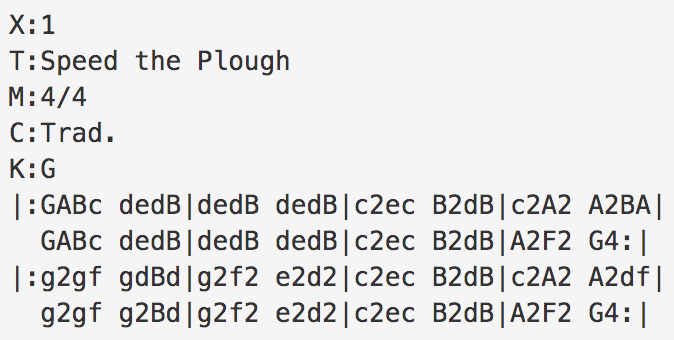
\includegraphics[scale=0.7]{abc-notation}
                \caption{Przykładowy zapis w\,\,notacji ABC}
                \label{abcnotation}
            \end{figure}

            Dużą zaletą tego formatu jest jego wysoki stopień kompresji. Za pomocą relatywnie krótkich ciągów
            znaków możliwe jest opisanie znacznej część utworu muzycznego. Głównym mankamentem notacji ABC
            w\,\,kontekście niniejszej pracy jest fakt, że nie wszystkie ciągi znaków są poprawnymi zapisami 
            w\,\,notacji ABC. Oznacza to, że pojedyncze błędy w\,\,generowanych sekwencjach mogą powodować niepoprawność całego utworu.
            W\,\,przypadku niemożliwości wyuczenia modelu tworzenia całkowicie poprawnych sekwencji niemożliwa byłaby
            transformacja dowolnej sekwencji do pliku midi. Chcąc zapewnić możliwość generacji utworów muzycznych
            konieczna byłaby walidacja i\,\,implementacja obsługi i\,\,poprawiania błędów w\,\,zapisie.
        }

        \subsection{Format midi}
        {
            Pliki w\,\,formacie midi są zapisem wiadomości przesyłanych protokołem komunikacyjnym o\,\,ten samej nazwie.
            Każdy plik midi składa się z\,\,kanałów oraz ścieżek. Poszczególne kanały reprezentują poszczególne instrumenty
            biorące udział w\,\,nagraniu. Na poszczególnych ścieżkach znajdują się wiadomości reprezentujące zdarzenia w\,\,utworze.
            Do najczęstszych z\,\,nich należą: note\textunderscore on, note\textunderscore off, set\textunderscore tempo.

            W\,\,przypadku wiadomości związanych z\,\,rozpoczęciem lub zakończeniem
            dźwięku dołączony jest również numer dźwięku z\,\,zakresu 0-127. 
            Wartości tego parametru odpowiadają kolejnym dźwiękom skali dwunastotonowej poczynając od C-1 i\,\,kończąc na G9.
            Dostępne dźwięki są nadzbiorem dźwięków dostępnych na 88 klawiszowej klawiaturze klasycznego fortepianu.

            Dodatkowym parametrem każdej wiadomości jest wartość time, będąca ilością taktów (ang. 'ticks') które upłynęły
            od poprzedniej wiadomości. Oznacza to, że długość trwania dźwięku można wyznaczyć poprzez zsumowanie parametrów time
            wiadomości występujących pomiędzy odpowiadającymi sobie zdarzeniami note\textunderscore on i\,\,note\textunderscore off.

            Możliwa jest konwersja wyznaczonej wartości zarówno na czas w\,\,milisekundach i\,\,wartości rytmiczne.
            Stałe potrzebne do tych przekształceń są naczęściej zawarte w\,\,meta wiadomościach znajdujących się na początku utworu.

            Zaletą formatu midi jest dyskretna reprezentacja wysokości dźwięku oraz pozwalająca na elastyczną 
            interpretację postać upływu czasu.
        }

        \subsection{Podsumowanie}
        {
            % Wszystkie omówione formaty danych mają wady i\,\,zalety. Cechą opisującą wszystkie z\,\,nich, jest 
            % bogata dostępność danych, przez co wybór dokonano na podstawie pozostałych cech.

            Wszystkie omówione formaty danych mają wady i\,\,zalety. 
            Ponieważ dostępne są zbiory utworów w\,\,każdym z\,\,przytoczonych formatów, wybór nie był ograniczony dostępnością danych, 
            a\,\,decyzja została podjęta na postawie ich cech.
            
            W\,\,dalszej części pracy opisywane podejścia będą tyczyć się jedynie plików w\,\,formacie midi, na którego 
            wybór zdecydowano się drogą eliminacji. Pliki audio odrzucono przez wymaganą złożoność wstępnej obróbki,
            a\,\,notację ABC z\,\,powodu obaw związanych z\,\,trudnościami zagwarantowania syntaktycznej poprawności 
            generowanych ciągów znaków.
        }
    }

    \section{Opis wybranego zbioru danych}
    {
        Do dalszych eksperymentów, opierających się na różnych sposobach tworzenia numerycznej reprezentacji
        danych wybrano stosunkowo mały zbiór zawierający utwory z\,\,serii gier Pokemon.
        Zbiór składa się z\,\,dziesięciu utworów o\,\,średniej długości wynoszącej 90 sekund. Kompozycje zawierają zarówno 
        elementy monofoniczne, jak i\,\,polifoniczne. Główną motywacją wyboru tego zbioru była jego mała objętość,
        co pozwalało na szybsze testowanie metod obróbki danych i\,\,procesu uczenia.
    }
}